\section{Background and Problem Formulation}\label{sec:model}
\subsection{From Augmented Trees to Temporal Maps}\label{sec:prior_pipelines}
\begin{figure}[H]
\centering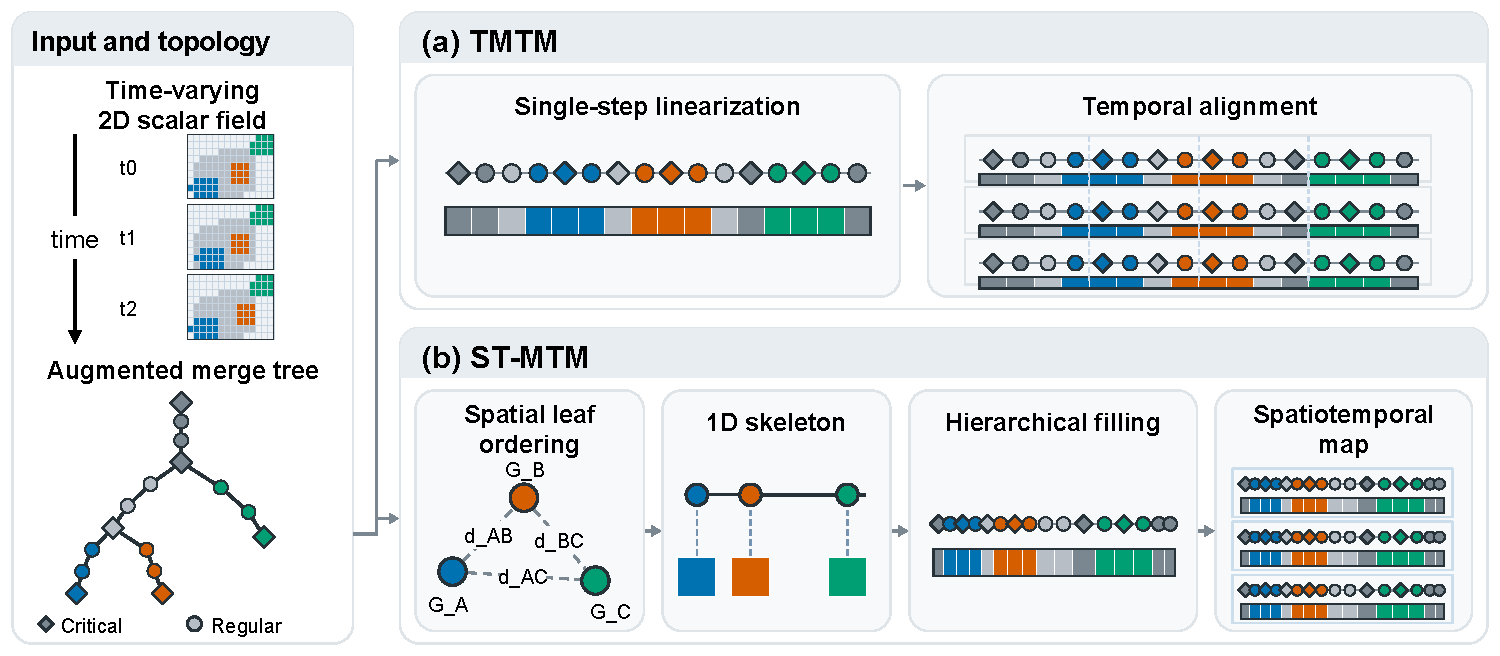
\includegraphics[width=\linewidth]{figures/Fig2.pdf}
\caption{Conceptual comparison of preceding merge-tree map workflows, redrawn and extended from ST-MTM Figs.~1 and 3~\cite{STMTM:2026}. Both use augmented trees with critical (diamond) and regular (circle) nodes. (a) TMTM~\cite{Koepp:2023:TMTM} linearizes samples within subtrees and optimizes temporal alignment. (b) ST-MTM constructs a distance-aware 1D skeleton, fills its scalar domain, and assembles the map. Branch/sample identities use the same palette throughout the schematics: $A$ (blue), $B$ (orange), and $C$ (green); internal groups are grey.}
\label{fig:prior_work}
\end{figure}

Figure~\ref{fig:prior_work} summarizes the two constructions on which RG-MTM builds. Both start from an augmented merge tree for each scalar-field observation. Critical nodes describe extrema and component merges; regular nodes retain samples along the arcs. The branching hierarchy groups connected scalar regions, while augmentation carries their values into the linearized field.

In TMTM, a recursive traversal maps all tree samples to a one-dimensional profile~\cite{Koepp:2023:TMTM}. Each subtree occupies a contiguous interval whose length is proportional to its sample count. Changing child order changes the linearization while preserving the merge tree. Temporal optimization selects these branch decisions to make interval overlaps between adjacent profiles agree with source-space subtree overlaps; stacking the aligned profiles produces the temporal map (Fig.~\ref{fig:prior_work}(a)).

ST-MTM separates geometric layout from scalar filling~\cite{STMTM:2026}. It first reorders leaves within the hierarchy using distances between feature centroids, then optimizes a one-dimensional skeleton to approximate feature distances under non-overlap constraints. Its temporal mode also uses tracked leaves to improve consistency between consecutive layouts. Leaf-arc sampling and hierarchical path filling populate the resulting intervals and gaps with scalar values before temporal assembly (Fig.~\ref{fig:prior_work}(b)). The diagram's lower path summarizes these stages; its temporal optimization acts during skeleton construction.

These constructions establish topology-preserving linearization and geometry-aware placement, respectively. Their admissible orders keep each subtree contiguous. A fixed spatial projection can instead request interleaved leaves from different subtrees, making reference alignment incompatible with that order constraint. RG-MTM diagnoses the resulting displacement, selects which constraints to retain or release, and measures the scalar cost of the chosen order. It reuses the augmented trees and scalar/path-filling framework while adding reference coordinates, positional certificates, and optimal barrier correction.

\subsection{Scalar Features and Merge Relations}
The input comprises processed fields $F_t:\Omega\rightarrow\mathbb R$, augmented merge trees $T_t$, leaf supports, and temporal matches. For a join tree, leaves are minima and internal nodes record the levels at which sublevel-set components merge. Split trees follow the same convention after negating scalar values. Augmentation retains regular samples along tree arcs, providing field context for the one-dimensional profile.

Leaf $i$ has extremum position $e_i^t$, value $f_t(i)$, support measure $\mu_i^t$, and support centroid $G_i^t$. The measure is area for a planar field and volume for a volumetric field. The extremum defines the positional reference; the centroid supplies the geometric distance term. Adjacent-frame support intersections define a maximum-weight Hungarian matching, with positive-overlap assignments continued as tracks.

Contracting unary chains gives the branching hierarchy for ordering. A legal permutation $\pi\in\Pi(T)$ keeps every subtree's leaves contiguous. For a join profile $\psi$, the merge level of two labelled extrema is the maximum on their inter-anchor interval $I_{ij}$. Its discrepancy from the source tree is
\begin{equation}
 d_{\rm top}(\psi,T)=\max_{i<j}\left|\max_{x\in I_{ij}}\psi(x)-f(\lca_T(i,j))\right|.
 \label{eq:merge_error}
\end{equation}
The original tree $T$ defines these targets; the ordering tree $T'$ defines admissible permutations; the filled profile $\psi$ is the measured output. A single-leaf frame has zero pairwise error.

\subsection{Reference Positions and Interval Geometry}
A fixed projection assigns $q_i^t=\langle e_i^t,d\rangle$ to one canvas $[a,a+L]$. Each feature receives a width $w_i=c\mu_i$, interval centre $z_i$, and extremum anchor $u_i$. Its eccentricity radius is $h_i=\rho w_i/2$. The interval must lie inside the canvas, consecutive intervals must leave a gap of at least $g$, and the anchor must remain within $h_i$ of its centre. Together these rules define the interval geometry $\mathcal G$ used by Algorithm~\ref{alg:rgmtm} and the layout in Section~\ref{sec:method}.

The width scale $c$, gap $g>0$, slack fraction $0\le\rho\le1$, and canvas remain fixed across time. Packing requires $\sum_iw_i+(n-1)g\le L$. Positive gaps separate the ordered anchors while allowing motion within their allocated intervals. Supplement S1 gives the complete linear constraints.

The primary position objective minimizes $\max_i|u_i-q_i|$. The scalar objective minimizes Equation~\eqref{eq:merge_error} with fixed extremum values. Temporal layout follows the projected displacement of matched extrema. These objectives connect source coordinates, scalar connectivity, and temporal evolution within one explicit display model.
